\chapter{An Approach for Reproducible Analysis}

A strategy is needed to facilitate reproducibility of NMR data analysis.
This chapter will describe in more detail the common characteristics of
the missing data and what role they play as well as why it is important to
capture them, a model for capturing that data, and a strategy for using
the model during the analysis process.


\section{Missing data and its role in analysis}

% need to cover what the data is, how it plays a role in NMR analysis, 
% why it's important to capture
As was described in earlier sections, 
spectral analysis, including peak picking, GSS construction, GSS and resonance
typing, sequential GSS assignment, and sequence-specific GSS assignment is 
accomplished using a step-by-step process of deductive reasoning 
which is often augmented by computational tools.  The computational 
results may be subject to manual validation, correction, and extension
\cite{guerry2011automated}.  This section will explore the various types
of data involved.

\subsection{Intermediate results}

An important feature of the analysis process is that the final results are
not the output of a single replicable step, but rather of a series of steps
of refinement and modification.  Thus, the analysis process implicitly 
generates a new data set (from the previous one) after every modification, 
whether manual or automated.

Implicit in the sequence of data sets are logical dependencies of derived
data upon features of the previous data set: the context of each deduction
is important, because the exact context determines what deductions may be
made and the confidence level of each deduction. % TODO an example

The importance of capturing intermediates is due to the dependence of 
deductions on context: without knowing the context, it is impossible to 
evaluate the correctness, confidence, and alternative interpretations of
a deduction.  In standard approaches to analysis, the contexts are not
captured; they are implicit.  By making the contexts explicit, it becomes
possible not only to fully recapitulate the process of analysis, but also 
to employ error detection and correction strategies by analysis
of deductions and their contexts.  
An interesting side-effect of capturing
contexts is that analysis can be restarted in the middle, by selecting an
appropriate context and applying a different deduction.
See Figure-\ref{deduction} for an illustration.

 - I can come up with a simple example that demonstrates: 1) the dependence of
   deductive ability on context, 2) the concept and utility of multiple 
   snapshots, 3) the concept and utility of tracking logical dependencies
% TODO 
% maybe an aspect of reproducibility is to make explicit what the variables,
% biases, input are.  so here, we're going to take the implicit context of
% deductions and make it explicit
 - importantly, today's final data set becomes tomorrow's intermediate

% TODO a paragraph on the significance of capturing these data
% must record intermediates, b/c it is not possible to recapitulate the 
% analysis process without a record of those intermediates

\subsection{Extraneous Results}
 - what: explicit identification of data features as being 'not of interest'
   to this analysis
   - peaks
   - resonances
   - GSSs
 - how it plays a role: if they're not identified, you could get: wrong 
   chemical shifts, wrong sequential GSS GSS, wrong GSS residue assignments
 - why: provides a marker for future perusers
 - allows separation of identifying a data feature vs. interpreting it -- which
   matters because the way we do things is self-consistent, right?  
   so if you have to come back and reinterpret -- and remember, PINE is great and the
   lesson is that you *will* have to reinterpret -- you won't have to reidentify
   features.  
   and that's *good*, because that means that your feature identification
   can be unbiased.  
 - provides additional context for estimating the quality of an analysis,
   where errors may be likely to come from (the borderline cases!), helps with
   assigning confidence levels to datums by not forcing it to be a binary 
   decision.  quality measures: \# of peaks found by peak-picker, \# of false
   positives, \# of additional peaks picked, \# of peaks assigned to GSS, 
   \# of GSS assigned to residue, etc.
 - also, reporting these gives measures of, perhaps, contamination,
   incompleteness, overcompleteness/overfitting, consistency.  
 - remember another
   lesson from PINE: there's a balance between false positives and false negatives,
   and if you want to avoid false positives -- which I think we usually do -- 
   you'll probably have some false negatives.  so they should be reported
 - the fact that a peak was found, and later interpreted as noise does 
   not show up in the final data set.


\subsection{Deductive reasoning}
 - examples: what are they?  NMR-domain-specific rules for analyzing data
 - examples: how do we use them?
 - examples: how is recording them useful (to others)?
   provides explanation of why something was done -- which adds semantic data
   to a deduction; this semantic data provides additional meaning, which can
   be used for checking, learning, etc.

\subsection{Notes}
 - examples: what are they?
 - examples: how are they useful?  facilitates future reinterpretation if
   additional data is made available.  similar to PINE -- use notes to mark
   low-confidence portions of analysis
   allows highlighting of known flaws, as well as indicating how a data set
   may be improved
 - could think of these notes as a generalization of PINE's confidence metric,
   b/c: score can contain more than just a number, can refer to more than just
   a single datum


\section{A Model for Reproducible NMR}

\subsection{Data models}
 - what is a data model, and how is one used?
 - enables formal communication
 - enables automated communication
 - makes semantics -- i.e. the meaning of the data -- interpret
 - abstract -- allowing multiple implementations
 - builds on BMRB and CCPN

\subsection{Extraneous results}

\subsection{Intermediate results}

\subsection{Deductive reasoning}

\subsection{Notes}


\section{An Implementation of the Model}


\section{Applying Reproducible Analysis}
 - what to do -- tips and suggestions to be effective
 - what not to do -- common roadblocks and problems
% maybe talk about the culture of the lab notebook?
% could this belong in its own chapter?
% or in the software chapter, or in the 'reproducible data sets' chapter?


\section{Archiving Reproducible Data Sets}
 - the NMR-Star file format, my parser, and others
 - the usefulness of NMR-Star files
 - the NMR-Star data dictionary
 - extending the NMR-Star data dic
 - other efforts to provide this NMR-Star integration ???


\section{Discussion}
 - lab notebooks
 - what data is missing
 - extending existing models to support these data
 - getting a handle on bias of data analysis
 - making things explicit


\section{Conclusion}
 - could go in with previous section


% figures
\clearpage
\section{Figures}

\begin{figure}[h]
  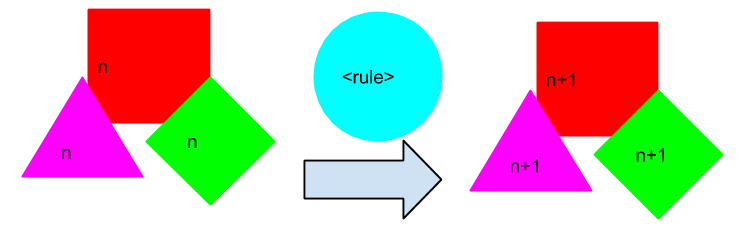
\includegraphics[scale=0.5]{figures/deduction}
  \caption[A deduction is a rule applied in a context]
          {A deduction is a rule (rounded rectangle) applied in a 
           context (circle), producing a new context (or data set).  
           If the context or rule is inapplicable, the deduction can
           not take place. }
  \label{deduction}
\end{figure}

